\documentclass[a4paper,15pt]{article}
\usepackage[utf8]{inputenc}

\usepackage{listings}
\usepackage{color}

\usepackage{hyperref}
\usepackage{csquotes}
\usepackage{graphicx}
\usepackage[english]{babel}
\usepackage[acronym, toc]{glossaries}
\usepackage[final]{pdfpages}

\setboolean{@twoside}{false}
%in the preamble
%--------------------------------
\usepackage[
    backend=biber,
    style=numeric,
]{biblatex}

\addbibresource{bibfile.bib}

\makeglossaries
\newglossaryentry{error-recovering}
{
    name=error recovering,
    description={Error recovering in parsers are the capacity of a parser to continue to parse as much as possible even if a error during the parsing occurs}
}

\newacronym{ide}{IDE}{Integrated Development Environment}

\graphicspath{ {resources/} }


%New colors defined below
\definecolor{codegreen}{rgb}{0,0.6,0}
\definecolor{codegray}{rgb}{0.5,0.5,0.5}
\definecolor{codepurple}{rgb}{0.58,0,0.82}
\definecolor{backcolour}{rgb}{0.95,0.95,0.92}

%Code listing style named "mystyle"
\lstdefinestyle{mystyle}{
  backgroundcolor=\color{backcolour},   commentstyle=\color{codegreen},
  keywordstyle=\color{magenta},
  numberstyle=\tiny\color{codegray},
  stringstyle=\color{codepurple},
  basicstyle=\footnotesize,
  breakatwhitespace=false,         
  breaklines=true,                 
  captionpos=b,                    
  keepspaces=true,                 
  numbers=left,                    
  numbersep=5pt,                  
  showspaces=false,                
  showstringspaces=false,
  showtabs=false,                  
  tabsize=2
}

%"mystyle" code listing set
\lstset{style=mystyle}
%--------------------------------

\begin{document}


\includepdf[pages=-]{chapter/cover.pdf}

% Title section
\begin{titlepage}
    \begin{center}
        \vspace*{1cm}
        
        \textbf{Kent Project Research: On-line parsing}
        
        \vspace{0.5cm}
        How to improve the speed of parsers in the treatment of big file in high frequency change context
        \vspace{1.5cm}
        
        \textbf{by PLATEL Kevin}
        
        \textbf{Supervisor: CHITIL Olaf}
        
        \vspace{1cm}
        
        A thesis presented for the degree of\\
        MSc Network \& Network Security
        
\includegraphics{uksc_logo}
        \vfill
        
        Computer Science Department\\
        University of Kent\\
        England\\
        March 2015
        
    \end{center}
\end{titlepage}

\newpage{}
% Abstract // TODO
\section{Abstract}
    Parsers are intensely use in many software and application for different purpose, one of this purpose is to provide useful and efficient software development tools and it's important for developers productivity to have tools that allow them to make a quick modification even inside important file as configuration file for example.\\
This research paper focus on the efficient aspect of parsers that are capable to react at each input (also called 'on-line' parser) without losing to much help features (auto-completion, error detection, ...) by analysing 2 big family of parsers, Bottom-Up and Top-down, and will look deeper in a possible combination of this 2 approach of parsing.\\
The global approach is that in the edition of important document section, the bottom-up approach can provide good performance where its the most needed, but the top-down approach can be better for little modifications and "hand-writing" code.\\
Implementing this kind of algorithm can be difficult, but it may open the research on tools or parsers to a new approach of algorithm combination and "context-aware" parsing.

% Index section
\renewcommand{\contentsname}{Table of contents}
\tableofcontents

\newpage{}

% Introduction
\section{Introduction}
During the past 50 years, we have seen an important increase numbers of computer and software everywhere in our society to speed up our everyday action as communicate, writing books, searching information, ... and this desire of speed up every action reflect also in work, to take an order, or managing planning, but the software development has not been forgotten, and it's even maybe from this sector that this willing to make process quicker comes from.
\\
In the past, software development would be a job for patient people because each compilation could take hours, so it's been a early concern for developers because it's annoying to find that you miss a semi-columns after 5 hours waiting, so a lot of technique have been created through time to speed up this process with incremental compilation to compile only the modified file or even interpreted language as python or ruby to run directly after a modification.
\\
\\
One big improvement of the software development process have been the parser with static (or dynamic) syntax analysis that check the validity of a program before and warn the developer if something he write is not valid in the language (or more with dynamic analysis). A lot of tools have been written but, as the software become more and more complex with more and more functionality, the size of these program increase too. This increase of size make the work of parsers more difficult as the amount of data to analyse become bigger and bigger and the time to analyse all of these data become slower and slower.
\\
\\
A lot of programming language analysis tools used in IDE, are based on one type of parser like top-down or bottom-up. Each of them have some advantage compare to another, even if generally top-down parsers are best to predict things, bottom-up parsers are quicker in most of the case, so each tools have to chose between these 2 approach and trade between speed and predicatively.
\\
\\
This choice is often made because this tools are based on the actual parser use in the compiler or interpreter of the language, and so re-create from scratch the parser can be difficult.
But it would be interesting to know if another approach of this problem is possible, and this research paper will analyse the problem and propose another approach of parsers inside IDE to offer a quick and predictive parser.
% Going more in precision
% Linter : use more parser than linter
    \subsection{Aims of the research}
    \subsubsection{Objectives}
This research will focus to figure out if it's possible to improve the speed of parsers in case of large file on active modification, assuming someone make some modification in the middle of the file. Parsers design to be used in this context are called "on-line" parser even if it's not an official appellation, it will be used in this paper.

This research will be split in 4 part :
\begin{itemize}
\item Analyse of actual state of the art of the research
\item Implementation of a parser base on this research
\item Design of a better theory model
\item Implementation of this solution and comparison with the previous implementation
\end{itemize}

This approach have been choose to make the result and the compare more sense. The 2 implementation of the parsing algorithm will be implement on the same base, so the comparison will be the most fair as possible and the result will not be influence by a possible programming language choice difference.
\\
\subsubsection{Context and precision}
The research will focus on the parser part of a linter, even if others optimisations are possible.
An others restrictions will be to work always in the context of "First run", so all the principle of cache file to improve the start up time will not be cover.


% Background
\section{Background}
Many techniques have been used to speed up development process through time on different sector of the development process, on the compilation through incremental compilation and compilation optimisation, and cache file to save result and computation time or, one of the main part of this tools, parser.
Many parsing algorithm exist but haven't necessarily think for the context of a IDE (Integrate Development Environment).
\\We will see different parsing algorithm and their advantage and disadvantage.
\subsection{Parser}
Before continuing further, an important point is to define what is a parser. A parser is a program that will take a input (usually a string) and will transform it into a structure more understandable by a computer program (usually a graph or a tree).\\

\subsection{Parsing technique}
One of the main part of a linters (or syntax analyser) is the parser. it's the principal part that will define the behaviour of tools, because a top-down parser will not allow the same thing than a bottom up parser.

\subsubsection{Context and Grammar}
First of all, a grammar is a set of terminal rules with terminal symbol (like characters) and non-terminal rules which are a set of terminal and non-terminal rules.
An important thing to know is the context where the parser will operate, and one big point is to know the grammar that the parser have to work with. 4 type of grammar exist\cite{grune2008parsing} and each type allow a grammar to be more or less ambiguous, which means that it's more or less simple to chose between 2 grammar rules with the same parsed information, and this "level" of ambiguity will define the difficulty to write the parser and the capacity of deductions.
\\In fact Context Free (CF) grammar \cite{cfg_def}, a grammar where the production rules is a single non-terminal rules that produce one or multiple terminal or non-terminal rules, are easier to parse and to give better feedback in case of error because it's simpler to predict what are the next possible symbol in this context \cite{grune2008parsing}, actually most of programming language are based on CF grammar, that allow syntax analyser to offer what's are called "Auto-completion" to developers. 

\subsubsection{Grammar}
As said above, grammar are an important component of parser and give most of the constraint the parser will have to manage. In fact, parse a URL and parse a complete programming language is not the same thing. First, a grammar is a set of rules, where each rules are describe by a set of rules on the left of the assignment operator, that will be produced if the set of rules on the right are present in the same order.\\
For instance, a rule can be described like "B ::= A 'a' 'b';", here B can be produced if the rule A and the character 'a' and 'b' are parsed. Another interesting thing is the difference between terminal and non-terminal rules. Terminal rules are rules where all the rules on the right are describe as character, here 'a' and 'b' are terminal but the rule B is not.\\
To describe this difference of complexity, All language are describe by different type of grammar, for example, an URL can be described with a grammar of type 3 and a programming language like Javascript can be described by a grammar of type 2. Researchers actually agree that all the grammar can be classified in 4 types from a grammar with recursivity inside the definition and with a mathematical proof that it's impossible to create a parser generator for this kind of grammar to grammar that are only defined by one terminal rule.\\
Grammar can be represented by different forms, like BNF (Backus-Naur Form) or CNF (Chomsky normal from) that are different ways of write and describe a grammar, some forms can impose some constraints, as CNF impose to eliminate right-hand sides with more than 2 non-terminals, and some algorithm transform some form to others to simplify the generation of parser or parsing table.\\
Even if a lot of the mathematical research is done on grammar and grammar type, some algorithm are still created to transform grammar and make them simpler or easier to use.

\subsubsection{Grammar Table}
Grammar table is a tool used by a lot of popular parsers today like LR or LL parser. Grammar table are table that associate a state with the next element parsed and the action to do. With this kind of table each time you parse an element and the actual state in the parser, you can know which action you have to do and the next state of your parser.\\
This kind of table are very interesting for parsers because in many case this table is generated and so it will be the exact same table for the same grammar. This pre-computation will be computation saved during the parsing and so better performance can be achieved. An other interesting point is the optimisation done during the generation, most of the grammar table are generated by transforming a table to a NFSA (Non Finite State Automaton) then to a FSA (Finite State Automaton), during this procedure, a lot of optimisation can be done, like removing impossible production rules, transform non-terminal to terminal rules, ...\\
Grammar table are a open field of research, each parser having its own table and focus on different aspect as predictability or performance.

\subsubsection{Top down}
Top down parser will try, at each symbol read, to create the whole syntax tree. Syntax trees are logical tree structure where each node store the parsed symbol and the syntactic rules it correspond, possibly based on which next symbol the parser can expect \cite{knuth1971top}\cite{grune2008parsing}. 
\\One of the most known top-down parser family are LL parsers. this kind of parser which are based on prediction and expectation, are really good when a parsing error occurs (often because it can not, or don't know how to, build the next node) to go back to a previous stable state or other prediction branch. This is call "error recovering"\cite{panopticoncentral_2009}. This can be exactly what we want of a good syntax analyser, the trade off in computation time to create all this syntax tree, specially when the user will modify intensively the file.

\subsubsection{Bottom up}
Bottom up parser are the opposite way of thinking. On each symbol, the parser will try to create a terminal token (a word, a keyword) and when the parser have a terminal token, it will try to "shift" these token to create an "upper" token\cite{knuth1971top}\cite{grune2008parsing}.
\\One of the most known bottom-up parser family of LR parsers. This kind of parser are more sensible to ambiguity because if in the step of shifting, the accumulate token can be transform in 2 "upper" token, the parser will fail. To prevent this behaviour a sub family of LR parsers called LR(*) are used. LR(*) parser ('*' is the token) will read one token, and if an error happens, the parser will read  more tokens to determine which rule make more sense. But for each other token read the complexity and the computation time increase, this is why the most used is the LR(1).
\\Bottom up parser are quick, but compare to top-down parser, it can be more sensible to errors even with LR(1), but with the today's technology, specially the increasing number of parallel process our CPU can handle a various of the LR and LR(*) parsers called GLR for "Generalise LR", where when the parser find a ambiguous situation and thread will be created for each possible syntax tree\cite{panopticoncentral_2009} and will kill the thread if it's impossible to resolve this scenarios. This algorithm shows really great performance and error recovering, but can use more resources.

\subsubsection{Incremental parsing}
Incremental parsing refer to parser which will try to detect each change made and will modify the syntax tree without recreate the whole tree.\cite{grune2008parsing}\cite{horspool1990incremental}
\\Every parsing algorithm can be modified to be used as "incremental parser", but they are often combined with a prediction algorithm to try improve the error recovering, because when you can predict what can happen next, you can pre-process and so improve the speed.
\\A technique used is to have 1 syntax tree and 1 linear representation of the data, and on each modification on the linear representation, the parser will try to modify the tree with the minimum impact and computation.

    
    \subsection{Related work}
    All this technique describe before about parsing technique for dynamic parsing or "on-line" parsing are use in many research field or application.\\
\subsubsection{Natural language}
A lot of the research about "on-line" parsing are about the parsing of what we can call "Natural language" or "human language", all this term refer to the parsing of English or French language. This research field is used in this context for application like Word or open office, where correction, prediction and specially because it's important, where treating big file, to not re-parse all the file on each modification.\\
\\
\subsubsection{Compilers}


% Approach
\clearpage
\section{Design}
This section will focus on the design of the algorithm and the implementation of the algorithm. It will describe the reflexion behind, the approach taken on the problem and the choice made for the implementation and describe the design of the algorithm

    \subsection{Reflection}
    After some research, we can see 2 important type of tools used inside of IDE for programming language analysis :
\begin{itemize}
\item The analyser and the parser are based on the language parser (parser used inside the compiler or interpreter of the language) as C++ with clang analyser \cite{Clang5:online} or Dartlang with dartanalyser\cite{darta0:online} or Golang with golinter \cite{golan5:online}
\item The parser have been "re-write" to feet in IDE requirement (as more prediction) and can offer to some tools or plug-ins inside the IDE the possibility to provide a grammar definition and some function will be "trigger" (called) by the IDE when the parser will find a element that match the provided grammar
\end{itemize}
In the first case, the tools use a parser adapted to the requirement of the language (error recovering or speed ...) but will not necessarily consider the use case of someone continuously typing some code, doing copy \/ paste of large block of code. This choice are perfectly adapted in the case of a compiler or a interpreter because you can assume the input code have to be correct and refuse and piece of code because it miss a semi-columns is perfectly normal.
\\
In the second case, the parser will try as most as possible to provide useful feedback to the developer by using a parser capable of predict what his expected next and with a large capability of error-recovering. This 2 factor are great for the developer (here the user) but, in some case, this features can slow down the parser. When it happen on 2 lines it's not really important, but when you paste a 50 lines of code in the middle of a big file it can slow down significantly the process (ex: The starting time of eclipse, or when you paste a lot of line inside eclipse)
\\
\\
So each technique have its advantage and its drawback, but a composite of the two can be a interesting solution to the problem of being the quickest as possible to provide feedback to the developer, when he make little or important edition inside a big or a small file.
\\
The idea is based on observation and research :
\begin{itemize}
\item Bottom-up algorithm are generally faster but less predictive
\item Top-down algorithm are generally more predictive but slower
\end{itemize}

So based on that, bottom-up algorithms can be more useful for big file or big edition inside a file, because it will treat all the information quicker and based on experience :
\begin{itemize}
\item When a important edition are made is often a paste from a other source where the syntax (not necessarily the variable name, ...) will be correct
\item When you open a big file, in lot of case a large part of the file will be correct, because it's have been generated, or because the developer (user) work on a piece of this big file and not all of them.
\end{itemize}

Top-down algorithms are very useful for error-recovering and prediction and so can give useful feedback and information to the developer. They are very powerful when working on smaller input, because base on experience :
\begin{itemize}
\item A lot of error made when programming are careless mistake, that can easily be corrected without the all context (the function context can be enough)
\item A prediction of what can be expect (or not) next can be very useful.
\\ example :
\begin{lstlisting}[language=C++, caption=simple prediction example in C]
// cursor after the '9' can expect '+', '*', '/', '-', '\%', ';'
int a = 9 
\end{lstlisting}
Here, a simplification of the prediction can be displayed as "next: 'mathematical expression' or 'end statement' " because a top-down algorithm will know which "node" can be expected next.
\end{itemize}
Based on this information, one path to explore can be a combination of the 2 algorithm based on the context by using the same syntax tree and collect as much as possible information during the parsing process.
    
    \subsection{Approach}
    To demonstrate my solution of algorithm combination, i will :
\begin{itemize}
\item Create a simple top-down parser from scratch
\item Create a bottom-up (a LR(0)) parser from scratch
\item Implement my solution with a combination of the 2 depending of the context
\end{itemize}

\subsubsection{Why re-create a parser from scratch ?}
I choose to implement 2 parsers algorithm for several reason :
\begin{itemize}
\item Be sure to understand the literature\\
Implement a parser and make it work will proof my understanding of the algorithm shown in the literature
\item Have the same base and language implementation to make the test "fair"\\
By implementing the parser myself rather than using a parser generator I'm sure that the comparison will be made on the same base (and possible mistake). So during the testing phase, any possible performance issue in the lexer (by example) will be shared, and so will have lesser impact on the result
\item Make the implementation of the solution quicker\\
The advantage by implementing the parsers by myself will be the possibility to use the same structure of syntactic trees, so the "merge" of the algorithm will be easier
\end{itemize}

\subsubsection{The algorithm : How it can work ?}
The approach of the algorithm is a little describe in the reflexion section.\\
The idea is to take the best of the 2 main type of algorithm in parsers today, top-down and bottom-up, and to take advantage of each one depending of the context.\\
The notion of context here is very important because it's this notion that will determine which algorithm will run the input.\\
\\
The choice is to consider bottom-up algorithm quicker on context-free grammar (the grammar type of almost all programming language), but less predictive by the nature of the algorithm.\\
And consider top-down algorithm slower than its bottom-up equivalence (like LL[0] for a LR[0]), but with the capacity to offer a better error recovering and more predictive than most of bottom-up algorithm.
    
    \subsection{Design}
    In the section, i will describe more deeply the algorithm i want to implement and the choice behind
\subsubsection{Taking care of the context}
One most important variable to take in count is the context where the algorithm will be run. On the context will depend the "mode" of the algorithm, actually 3 context will be treated :
\begin{itemize}
\item Opening the file: \\
This context is during the first read of the all file
\item small edition in the file ( \( buffer < 500 character\) )\\
This context is mostly during a small copy\/paste or during simple edition (keystroke)
\item Important edition in the file ( \( buffer >= 500 character\) )\\
This context is mostly during big copy\/paste
\end{itemize}

To know this context every time, i will have :

\begin{itemize}
\item Record where am i in the file ( character number n, line number l )
\item Update the position of each node inside the syntax tree every time a modification are made
\item Record the number of pending character inside the reading buffer
\end{itemize}
This will allow me to know which part of the file have been modify, and where the modification has been made.\\

\subsubsection{Parse the smallest amount of data}
An other part of the algorithm will be to limit the input treated by the algorithm. An easy solution when the user insert a new character is to apply the parser on the all line, but in some case it's not necessary and maybe only a part of the line can be re-parser.\\
example :
\begin{lstlisting}[language=C++, caption=parsing optimisation in C]
// inserting 2 here
//           |
//           v
int a = 9 * 82 / 53;
\end{lstlisting}
TODO : create schema of a syntax tree of this expression \\
in this expression, the syntactic tree will show that if a modification happen between character '*' and '\/', the node impacted is '8', so before run the parser on the all line, the algorithm will run the parser on the smallest sub-syntactic tree possible to know if it's possible to resolve the input.

\subsubsection{Running the right parsing algorithm}
Knowing in which context i am, the aims will be to run the top-down or the bottom-up algorithm depend of the context.
\begin{itemize}
\item If it's the first read of the file or during a important edition : run the bottom-up
\item If it's a small edition : run the top-down
\end{itemize}

The first read will create the general tree, then tree created during the top-down will be insert inside the main tree and during important modification, the all file will be re-parse.\\
The choice to re-parse the all file during important modification is made because implement a more clever algorithm will be to much time consuming but other technique exist, as try to create a sub-tree with a bottom-up approach and then try to insert the sub-tree inside the main tree

% TODO : create syntax tree of this expression

    
\clearpage
\section{Implementation}
During my research, I have implemented some algorithms found during my research and implemented some of mine to create the design solution described above. In this section, I will explain and review some of the functionalities developed, why I implemented those functionalities and how I implemented them.
\subsection{Technology}
To implement all this algorithm I chosed to use Dart, which is a language developed and released recently by Google. Dart has the advantages to be used inside a command line interface (as a shell as we can use python script) or to be compiled to JavaScript for being used inside a website or a browser.\\
One of my idea was to develop the solution and then offer a website where it could have been possible to test the implementation directly.

\subsection{Lexer}
The lexer is the part, inside a parser, that will handle the first action of a parser : transform input characters into tokens. A simple definition of a token, in a parser, is a set of characters or tokens identified by a specific key, by example the token 'digit' will identify all the characters considered as digit as 0, 1, 2, ...\\
This task is done by Scanner. Scanner is a class that will handle the process of taking a parsing unit (here a character) inside a input (a string or a file) and return a ParseUnit object that will store all the information about the parsed character as :
\begin{itemize}
\item its line inside the input
\item its position inside the line
\item its position inside the input (number of characters)
\item the parsed data
\end{itemize}
All this data can be used to give useful information to the user, and can also be used inside the designed algorithm to limit the information to re-parse. Knowing where the input is made can be interesting but requires to update all the parsed information and specially their position inside the file. Scanner will also skip some element (as space, tabulation or new line character) by default, but this option can be turned off.\\
All the concept of line, space, etc. are configurable through the ScannerConf object that can be pass during the construction of a Scanner object.

\subsection{Grammar construction}
One important point of a parser, is the treatment of a grammar. During the implementation my first approach has been to create a grammar through the overloading of operator mechanism of the Dart language.\\
So inside the parserflow project, a grammar can be describe as :
\begin{lstlisting}[language=C++, caption=Rules creation]
// Final rules.  ------ Sub rules --------
// |             |           Operator    |
// |             |         |         |   |
// v             V         v         v   v
Rules r = ((isMathOperator & isNum) | isDigit);
\end{lstlisting}
Here, 'r' is defined as "if the input match isMathOperator rules AND isNum rules OR isDigit rules". This way of describing the grammar offer several advantages for the user of this library and for me to create the grammar.
\begin{itemize}
\item it allows the user to simply describe a grammar
\item it allows a simple re-use of some more complex rules
\item it allows me to simply create a tree from this input
\end{itemize}
After each use of an operator, a new Rules is created containing the the type of operator with the 2 rules as child of this 'main' rules.\\
A Rules is defined by severals attribut as :
\begin{itemize}
\item A matcher function that will check if the input match this rules
\item A Quantifier that will describe how many times the matching function need to match to determine if the rules match the given input. As example, a number is described by AT LEAST ONE digit, but it can be more than one.
\item A list of possible child
\end{itemize}
With all this parameter, it's possible to define more complex grammar and the definition of the grammar will be close to the definition of a grammar with the BNF syntax.

\subsection{Grammar analysis and transformation}
During the process of implementation of the LR parser, my first difficulties have been to transform my grammar, represented as a tree, to a CNF grammar, base of a lot of algorithm to generate a parsing table.\\
So I had to implement a algorithm to transform a tree of rules to a CNF grammar, inside the implementation. It's done like that :
\begin{lstlisting}[language=C++, caption=Transform grammar to its CNF representation]
  // Grammar definition --
  var number = ((has('0') | has('1') | has('2'))["+"])..name = "num";
  var operator = (has('+') | has('-'))..name = "operator";
  var operation = (number & (((operator & number)..name="op")["*"]))..name = "operation";

  var expr = operation;
  var grammar = new CNFGrammarGenerator().generateGrammars(expr); // Creation of the CNF representation of the grammar
  print('grammar: ${grammar}'); // print the the grammar is CNF style
\end{lstlisting}

The base of this algorithm are mainly based on equivalence of representation of a rules to its CNF representation. for example, a OR, describe in a BNF by "R ::= A | B" will be transform to "R ::= A; R ::= B". Here we can see that one production rule has been transform by 2, with 2 different right-hand rules. This nuance are on of all the differences we can found between a BNF grammar and a CNF grammar, but this differences are important because in the CNF syntax, the complete grammar tend to be bigger. But each rule will be simpler and with less "ambiguity" because the maximum amount of right-hand rules will be 2 without any quantifier or 'OR'.

\subsection{Grammar table}
As describe in the section about grammar table, these are key points of the most performing and used parsing algorithm today, principally because it allows to do pre-computation and detect then remove the maximum of errors in the previous grammar.\\
I had to implement the creation of a grammar table for a LR(0) parser, but to do so I had to transform my CNF grammar to a Non-deterministic Finite Automata (NFA) and then transform it to a Determine Finite Automata (DFA). The NFA is generated with the "walk the dot" algorithm. The input is the CNF grammar, by example this grammar :

\begin{lstlisting}[language=python, caption=example CNF grammar]
AB -> A     # rule 1
A  -> ( A ) # rule 2
A  -> a     # rule 3
\end{lstlisting}

Then, for each production rules, we will put a dot, before the production then after the next rules, etc. as describe in this example :

\begin{lstlisting}[language=python, caption=example of the "walk the dot" algorithm]
AB -> . A     # from rule 1
AB -> A .     # from rule 1
A  -> . ( A ) # from rule 2
A  -> ( . A ) # from rule 2
A  -> ( A . ) # from rule 2
A  -> ( A ) . # from rule 2
A  -> . a     # from rule 3
A  -> a .     # from rule 3
\end{lstlisting}

This operation will create a graph, with a link between each "state", this link will be use after to create the table.\\
To create the table, we need to go through each link of each node, and depends of the actual state and the next, determine which action will be the next and which state inside the table will be the next.\\
\begin{figure}[h]
\centering
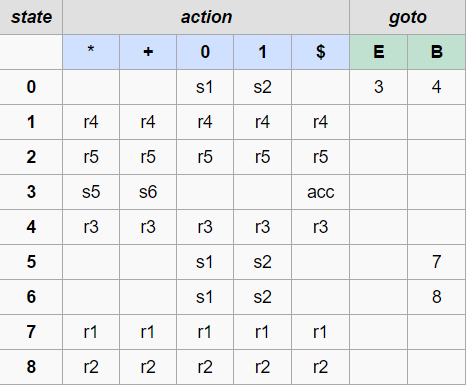
\includegraphics[width=0.5\textwidth]{LR-Table}
\caption{Example of LR grammar table. \cite{wikilr:online} }
\end{figure}
Generate this table, even if it can describe simply, was an important challenge and required a important effort. The current implementation works for simple case, but can produce wrong output for more complex grammar, even if it looks simple at first sight.

\subsection{Bottom-up parser : LR(0) Parser}
To implement my algorithm I had to implement a bottom-up parser. My choice was to implement a LR parser, principally because it's a key algorithm in most tools today, with a lot of variant as SLR, LR(1), LALR, GLR, ... \\
LR is the acronym for "Left input - Rightmost derivation" this kind of parser are really good to parser deterministic (at each state, we know which will be the next expected input) context free grammar and are mainly based on a grammar table as shown in the figure 1 and a stack\\
At each step, the stack will store the parse input and the state, so a stack in a LR parser can looks like :
\begin{lstlisting}[language=python, caption=example Lr parser stack]
stack = ['+', 1, '0', 0] # example of stack  
\end{lstlisting}
At each state, and in function of the parsed input the LR parser will know which action it have to do. Very few operation are done by a LR parser:
\begin{itemize}
\item Shift (ex: s1) : Shift (put the parse element in the stack) and push the state (here 1)
\item Reduce (ex: r1) : The reduce operation will remove element on the stack corresponding of the right-hand element of the rules indicate. (in the example the rule 1) and will look at the "goto" section on the table to know which state in the next
\item GoTo (ex: g3) : After a reduced operation, the next operation is a "go to" operation that will push the next state corresponding of the reduce rules. For example inside the figure 1, after a reduced operation that makes the parser go back to the state zero, the next state of the parser will be 3 if the reduce rules was E or 4 if it was B
\end{itemize}
This 3 operations are enough to parse any input, but the main work is done by the grammar table which know what to do next in function of the state and the next input.\\
This kind of parser is simple to implement IF the grammar table is provided, but the generation of the grammar table was a real challenge. Inside the implementation this algorithm work correctly for a correct grammar table.

\subsection{Top-down parser}
The top-down parser was easier to implement because I chose to implement a simpler parser than a LL one. I chose to implement the most basic top-down parser.\\
This implementation works pretty well, and can be used like this :
\begin{lstlisting}[language=java, caption=top-down parser example]
  var number = ((has('0') | has('1') | has('2'))["+"])..name = "num";
  var operator = (has('+') | has('-'))..name = "operator";
  var operation = (number & (((operator & number)..name="op")["*"]))..name = "operation";

  var expr = operation;
  var input = "12+2-1";
  var res = expr.check(input);
\end{lstlisting}

The current implementation rely on the grammar tree created. Each rule node have a 'check' method that allow to verify that the input match the rules, but if the node has a child, it will check its child first, and the child will check its own child, and so on... This will give the base of the top-down parsing algorithm. A better description of the algorithm used is :
\begin{lstlisting}[language=python, caption=top-down pseudo code algorithm]
 input = range of input between nb character match and the end of the input
 node = get next node
 nb_match = 0
 check match in child
 IF child match:
   check node match
   IF node match
      nb_match += 1
 IF nb_match is in node quantifier range:
   GO TO 4
 ELSE IF nb_match match node quantifier:
   RETURN number of character match
 ELSE:
   RETURN match_fail
\end{lstlisting}
 At each step, a MatchInfo is returned, storing all the information about the match as the number of character match, the rules who has been matched, the match input, ... This information are used to know the parser location inside the input, and to construct the syntax tree.\\
The main difference with a bottom-up algorithm is the starting point, in a bottom-up algorithm, the grammar is checked starting by the terminals rules, but in a top-down, the first rules checked is the root (or goal) rule.
 
\subsection{The combination algorithm}
The main idea was to combine this 2 algorithms depending of the context, sadly due to the complexity of implementing the LR algorithm and the time required in research to transform the grammar and generate the table was too much to allow me to correctly implement this algorithm.\\
All the pieces are here, the MatchInfo node allow me to know the location of each parsed information in the input, the size of the match, and so apply the potential correct algorithm. One of the challenge was to be able to generate the exact same tree, so it would have been possible to use one or the others in a seamless way.\\

\subsection{Missing \& Future functionality}
The actual implementation is not complete, due to some reason main features are not available :
\begin{itemize}
\item On-line edition
\item Research algorithm
\end{itemize}
This functionality has not been implemented due to the unexpected amount of time in research, test and comprehension some part of this project have required. The part on the grammar was a really hard part because grammar by itself is an entire field of research and the manipulation of the grammar to transform a syntax to an others is a complete field.\\
I have underestimate some part of the implementation too, as the time required to allow an "on-line" edition and so make the appropriate modifications to the syntax tree.

\clearpage
\section{Analysis \& Result}
In this section, we will see the result of the implementation compare to the expectation.

\subsection{The test}
The test was supposed to be the edition of a big file (more than 5MB) and measure several times :
\begin{itemize}
\item Start-up time (after all the file have been parsed)
\item Little edition (\( <5 entry\)) at the beginning of the file
\item Important edition (\(> 200 entry\)) at the beginning of the file
\item Little edition (\( <5 entry\)) at the middle of the file
\item Important edition (\(> 200 entry\)) at the middle of the file 
\end{itemize}
With 3 case of study : One with a bottom-up parser (LR), one with a top-down parser, and one with my algorithm.

\subsection{The result}
No result are available because the implementation hasn't been finished.\\
The expected result was to show a better start-up time with the bottom-up algorithm and globally a better time for little edition for the top-down algorithm, but with a good average of my algorithm and a better performance for important edition.



\clearpage
\section{Conclusion}
Parsers are everywhere and are the bases of all the innovation of today, and on-line parsing will be a key point for future innovation. In a world where the amount of information treated increase and the need of speed is crucial, been able to give a quick feed back to the user or just been able to treat new information without re-do operation is very important.\\
In this research I have try to focus on the merge of best known parsing algorithm used today, I didn't succeed to implement my algorithm, but I personally think that research on parsers have reach a point where all the family of parsers have been found. As said by the authors in the second edition of 'Parsing Techniques: A Practical Guide' in the preface of their book :
\\
"If there will ever be a third edition of this book, we expect it to be substantially thinner. The reason is that the more parsing algorithms one studies the more they seem similar, and there seems to be great opportunity for unification."\cite{grune2008parsing}
\\
And the next possible innovation can be the fusion of the advantage of this different parsing algorithms.

\section{Future work}
The research in on-line parsing can be done on several aspects. During my research I have look at how take the good parts of bottom-up and top-down parsers to improve the speed of the parser but still have some prediction through the top-down algorithm.\\
Other fields of study could be the prediction accuracy, the syntax modification and insertion optimisation, prediction algorithm to predict common errors made by the user and so influence the choice of the top-down algorithm and get a more accurate prediction.\\
The area is still open and the popularity and new discoveries made in genetic algorithm could be a way to improve the tools by making them more aware of the user particularity.

\clearpage
\section{Link \& Resources}
\subsection{Parsing library}
\href{https://github.com/platelk/parserflow}{Link to the repository of the parsing library use}
\\https://github.com/platelk/parserflow
\subsection{Dissertation}
\href{https://github.com/platelk/On-line-parsing}{Link to the repository of the dissertation}
\\https://github.com/platelk/On-line-parsing

\section{References}
\nocite{*}
 
\printbibliography

\end{document}
